% example.tex
\documentclass[dvisvgm]{standalone}

\usepackage{amsmath}
\usepackage[usenames,dvipsnames]{xcolor}
\usepackage{tikz}
\usetikzlibrary {arrows.meta,
                 positioning,
                 shapes.geometric}

 \tikzset{
        base/.style={draw, align=center, minimum height=4ex},
        proc/.style={base, rectangle, text width=8em},
        io/.style={trapezium, trapezium left angle=70, trapezium right
                   angle=110, draw, text width=8em, %minimum width=2cm, 
                   %minimum height=1cm
                   },
        test/.style={base, diamond, aspect=2,
                     %text width=5em
                     },
        term/.style={proc, rounded corners},
        myarrow/.style={-Stealth, line width=0.25mm},
 }

\begin{document}
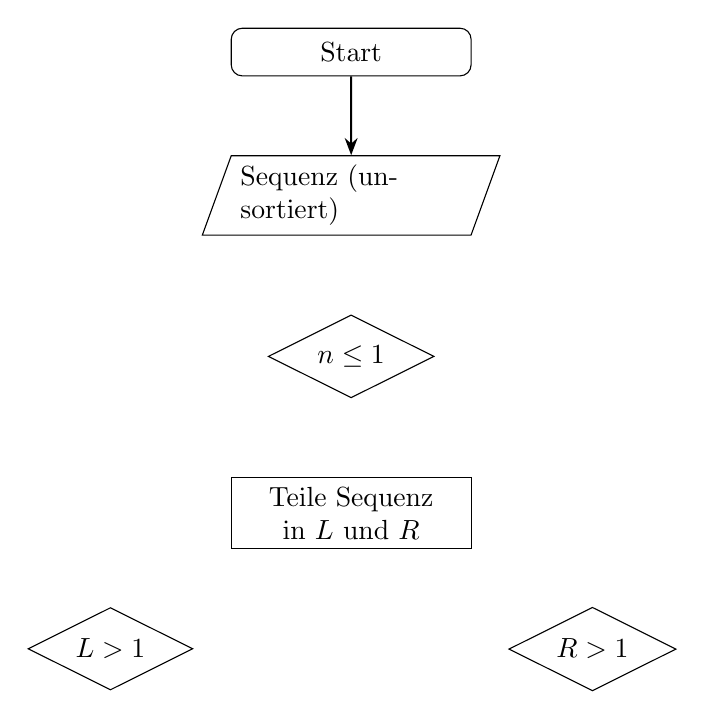
\begin{tikzpicture}
    \node[draw, term] (a) {Start};
    \node[draw, io, below= of a] (b) {Sequenz (unsortiert)};
    \node[draw, test, below= of b] (c) {$n\leq 1$};
    \node[draw, proc, below= of c] (d) {Teile Sequenz in $L$ und $R$};
    \node[draw, test, below left= of d] (e) {$L > 1$};
    \node[draw, test, below right= of d] (f) {$R > 1$};

    \draw[myarrow] (a) edge (b);
\end{tikzpicture}
\end{document}
